\section{Results}
  % Here the results of our study, within the bounds of our study only, should be discussed - times, most effective distributions, potential reasoning as to why.
  % The next section handles the relation of this to the real world.
\subsection{Control Results}
To test our system had the expected behaviour we ran a set of simulations with no food being generated in the map. In these simulations expected that the ants would forage for food until they had lost enough energy to need to return to the colony. At this point they would not be able to regain energy so they would half the amount of energy required before returning to the colony and forage again. This process would repeat until the ants `died' at which point there would be no ants left. This occurred as expected, video of this can be found at \url{https://www.youtube.com/watch?v=mHyaiDkegGc}

\subsection{Main Results}

As already described, the length of each simulation is 1200 iterations and the environment is set to a fixed 50x50 tiles for each run. The independent variable of this experiment is the percentage of major and minor workers. Given the stochasticity in our system, we took the average of 5 runs, with 5 separate seeds (1:5), for value in the experimentation. The average runtime of each run in an experiment was 255\si{s}. However all of the results were generated using Matlab's parallelisation ability where multi-core CPUs can be leveraged (more detail on this in Appendix D).\par
The results of our experimentation can be seen in the line graph in figure \ref{fig:iters-line}. There are 12 lines on this plot, 35\% represents the `natural system' value taken from the literature \cite{Tschinkel1988} and the rest 0-100\% in steps of 10 represent our experimental values. As you can see in the figure \ref{fig:iters-line} the natural system produces the 'best' result in terms of overall colony energy. This can also be seen in the bar chart of the same data found in Appendix C figure \ref{fig:iters-bar}.\par

\begin{figure}[H]
  \centering
  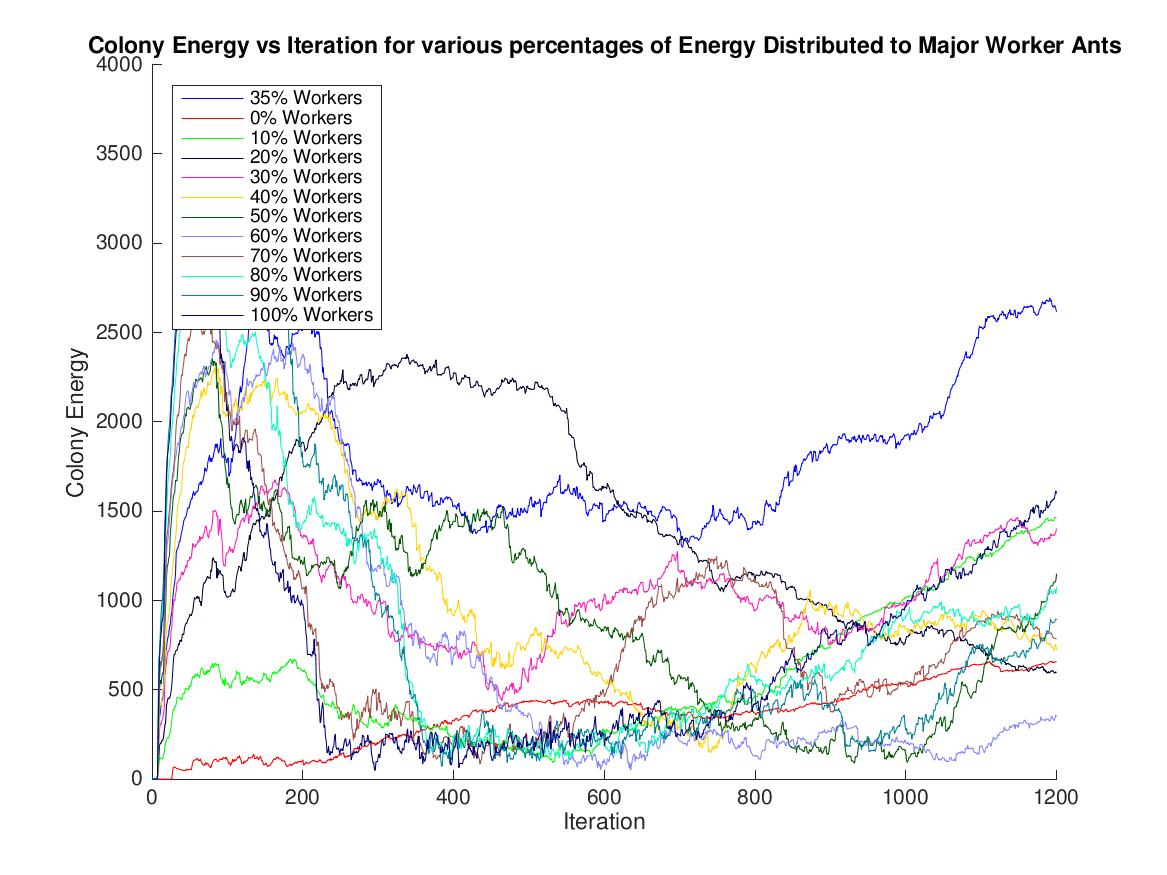
\includegraphics[width=1\textwidth]{images/line-graph-results.png}
  \caption{Line graph depicting colony energy against iterations (time) for various percentages of Major Worker Ant.}
  \label{fig:iters-line}
\end{figure}

This positive result around the value that the internationally renowned Professor Tschinkel's journal article \cite{Tschinkel1988} motivated further experimentation around the values between 30\% and 40\% of the colony being major workers. The values for this experiment were \{30\%, 32\%, 35\%, 38\%, 40\%\} The results for this are in the bar chart in figure \ref{fig:bar-chart-detail}. We were expecting a distribution that looked Gaussian around 35\% but this shows that the peak for our model is at 32\%.\par
A visualisation of our system can be viewed at \url{https://www.youtube.com/watch?v=tgsPYGt2TbI}. This is at the optimal ratio of major:minor workers for our system of 32:68 and runs for 1200 iterations which equates to 20 hours. 

\begin{figure}[H]
  \centering
  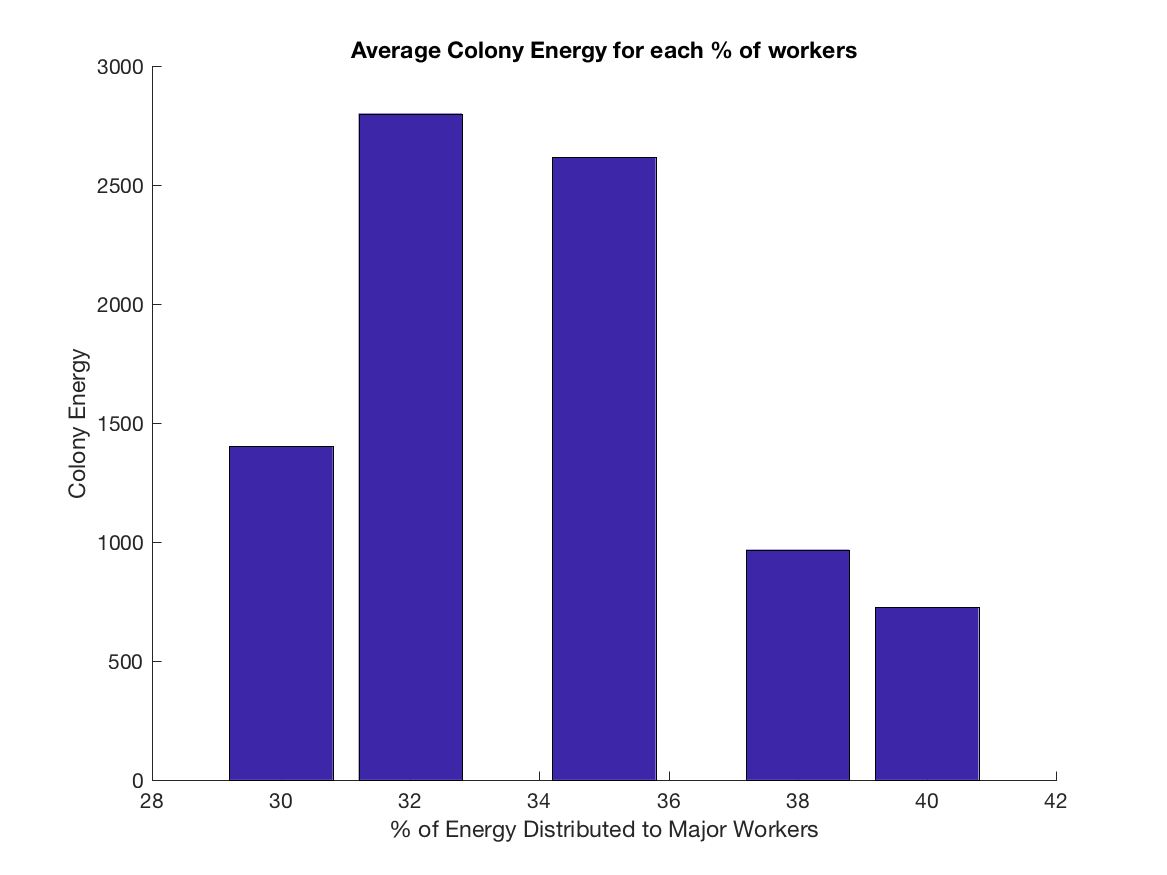
\includegraphics[width=0.6\textwidth]{images/bar-chart-detail.png}
  \caption{Bar Chart of more detailed experimentation based on positive results between 30\% and 40\%}
  \label{fig:bar-chart-detail}
\end{figure}
 
\subsection{Computational Efficiency}

When running the simulation with graphics enabled the largest portion of computation is spent on drawing the simulations results. In order to find bottlenecks in the simulation itself the profiler was used with the graphics disabled, to give a time plot table of what functions are the most expensive during the running of an entire simulation. Appendix B, figure \ref{fig:appendix1} shows the summary of the system and figure \ref{fig:appendix2} of the same appendix shows that the environment is the place where most computation happens.\par

 \begin{figure}[htb]
  \centering
  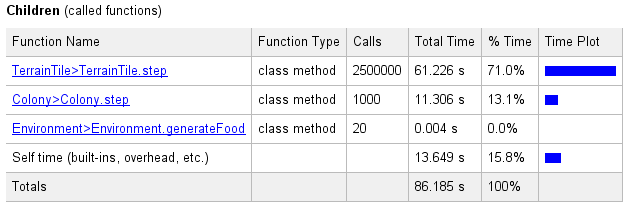
\includegraphics[width=0.8\textwidth]{images/text1.png}
  \caption{Profiling for the child functions of Environment - Environment.step}
  \label{fig:text1}
\end{figure}

 \begin{figure}[htb]
  \centering
  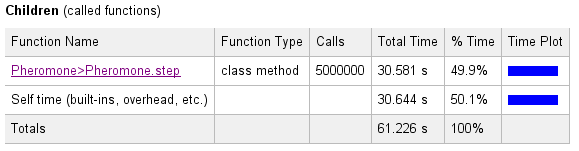
\includegraphics[width=0.8\textwidth]{images/text2.png}
  \caption{Profiling for the child functions of TerrainTile - TerrainTile.step}
  \label{fig:text2}
\end{figure}

When overviewing the computational costs of the environment step, it's highlighted in figure \ref{fig:text1} that the terrain tile is where the large majority of time is spent. As shown in figure \ref{fig:text2}, a large amount of the computation that is done during the simulation of the terrain tile is a result of the pheromone step function. As a result, it can be seen that the pheromone step is taking a large amount of computation to run, the reason for this being so expensive is that each tile of the map contains a pheromone which is then updated each timestep of the simulation. Running it this way means that tiles without active pheromones will still be receiving updates each timestep. However, a way of improving this to greatly reduce computation would be to instead keep a list of active pheromones and then only update those inside that list. When a pheromone decays to zero strength, the pheromone can be removed from the list and won't be unnecessarily updated each timestep.\par

\subsection{Repeatability}
Our results are fully repeatable. See Appendix D for a more in-depth view of this and how to run the system.\par
